\documentclass{beamer}
\special{landscape}

\usetheme{Warsaw}

%\usecolortheme{seahorse}
%\usefonttheme[onlysmall]{structurebold}

\setbeamertemplate{headline}[split]
\setbeamertemplate{footline}[default]
\setbeamertemplate{footline}[miniframes theme]
%\logo{\includegraphics[scale=0.25]{lifia_logo.png}}

\mode<presentation>
\usepackage[spanish]{babel}
\usepackage{beamerthemesplit}
\usepackage{color}      % use if color is used in text

\usepackage[utf8]{inputenc}

% Comandos en modo Verbatim
%\usepackage{fancyvrb}

\usepackage{listings}


\lstdefinelanguage[mips]{Assembler}{%
  sensitive=false,%
  morecomment=[l]{;},%
  % so listings can detect directives and register names
  alsoletter={.\$},
  % strings, characters, and comments
  morestring=[b]",
  morestring=[b]',
  morecomment=[l]\#,
  numberstyle=\color{green},
  % instructions
  morekeywords={[1]cvt.l.d,cvt.d.l,mfc1,mtc1,DADD,DADDI,ANDI,XORI,HALT,BEQ,BNEQ,LD,NOP,DMUL,DSUB,AND,DDIV,%
	JAL,J,DSLL,BNEZ,SD, JR, BEQZ, cvt.d.l, cvt.l.d, lwu},
  % assembler directives
  morekeywords={[2].word,.code,.data, .asciiz, .ascii, .word32},
  % register names
  morekeywords={[3]F0,F1,F2,F3,F4,F5,F6,F7,F8,F9,F10,F11,F12,F13,F14,F15,F16,F17,F18,F19,%
    F20,F21,F22,F23,F24,F25,F26,F27,F28,F29,F30,F31,%
    f0,f1,f2,f3,f4,f5,f6,f7,f8,f9,f10,f11,f12,f13,f14,f15,f16,f17,f18,f19,%
    f20,f21,f22,f23,f24,f25,f26,f27,f28,f29,f30,f31,%
    R0,R1,R2,R3,R4,R5,R6,R7,R8,R9,R10,R11,R12,R13,R14,R15,R16,R17,R18,R19,%
    R20,R21,R22,R23,R24,R25,R26,R27,R28,R29,R30,R31,%
    r0,r1,r2,r3,r4,r5,r6,r7,r8,r9,r10,r11,r12,r13,r14,r15,r16,r17,r18,r19,%
    r20,r21,r22,r23,r24,r25,r26,r27,r28,r29,r30,r31,%
	\$0,\$zero,\$s0,$s1,$s2,$s3,$s4,$s5,$s6,$s7,$sp,$ra,$t0,$t1,$t2,$t3,$t4,$t5,$t6,$t7,$t8,$t9,%
	$sp,$a0,$a1,$a2,$a3,$v0,$v1%
    },
  keywordstyle=\color{green},
  keywordstyle=[2]\color{blue},% for example
  keywordstyle=[2]\color{blue},% for example
  keywordstyle=[3]\color{red},% for example
 }[strings,comments,keywords]


\definecolor{CommentGreen}{rgb}{0,.6,0}
\lstset{
   language=[mips]Assembler,
   escapechar=@, % include LaTeX code between `@' characters
   keepspaces,   % needed to preserve spacing with lstinline
   basicstyle=\footnotesize\ttfamily\bfseries,
   commentstyle=\color{CommentGreen},
   stringstyle=\color{cyan},
   showstringspaces=false,
   keywordstyle=[1]\color{blue},    % instructions
   keywordstyle=[2]\color{magenta}, % directives
   keywordstyle=[3]\color{red},     % registers
%  numbers=left,
%  numbersep=15pt,
%  numberstyle=\tiny\color{green},
 }

%%
%% WinMIPS64 definition (c) 2020
%\lstdefinelanguage{WinMIPS64_old}
% {keywords={%
%cvt.l.d,cvt.d.l,mfc1,mtc1,DADD,DADDI,ANDI,XORI,HALT,BEQ,BNEQ,LD,NOP,DMUL,DSUB,AND,DDIV,%
%	JAL,J,DSLL,BNEZ,SD, JR, BEQZ, cvt.d.l, cvt.l.d, lwu},%
% otherkeywords={.word,.code,.data,.code, .asciiz, .ascii, .word32 },%
%   sensitive=false,%
%   morecomment=[l]{;},%
%   morestring=[b]",%
%   keywordstyle=\color{green},
%  keywordstyle=[2]\color{brown},% for example
% }

%\lstset{emph={%
%    F0,F1,F2,F3,F4,F5,F6,F7,F8,F9,F10,F11,F12,F13,F14,F15,F16,F17,F18,F19,%
%    F20,F21,F22,F23,F24,F25,F26,F27,F28,F29,F30,F31,%
%    f0,f1,f2,f3,f4,f5,f6,f7,f8,f9,f10,f11,f12,f13,f14,f15,f16,f17,f18,f19,%
%    f20,f21,f22,f23,f24,f25,f26,f27,f28,f29,f30,f31,%
%    R0,R1,R2,R3,R4,R5,R6,R7,R8,R9,R10,R11,R12,R13,R14,R15,R16,R17,R18,R19,%
%    R20,R21,R22,R23,R24,R25,R26,R27,R28,R29,R30,R31,%
%    r0,r1,r2,r3,r4,r5,r6,r7,r8,r9,r10,r11,r12,r13,r14,r15,r16,r17,r18,r19,%
%    r20,r21,r22,r23,r24,r25,r26,r27,r28,r29,r30,r31,%
%	\$0,\$zero,\$s0,$s1,$s2,$s3,$s4,$s5,$s6,$s7,$sp,$ra,$t0,$t1,$t2,$t3,$t4,$t5,$t6,$t7,$t8,$t9,%
%	$sp,$a0,$a1,$a2,$a3,$v0,$v1%
%    },emphstyle={\color{red}\bfseries}%
%}%

%\lstset{emph={%
%    .code,.data,.word
%    },emphstyle={\color{green}\bfseries}%
%}%

\title{Practica 6 - WinMIPS64}
%\author{Juan Antonio Zubimendi\\azubimendi@lifia.info.unlp.edu.ar}

\AtBeginSection[]

\begin{document}

\section{Atascos}


\begin{frame}
\frametitle{Atascos}
Llamamos \emph{atasco} a la situación que impide a una o mas instrucciones seguir su camino en el cauce.

\begin{itemize}
\item Estructural
\begin{itemize}
\item Provocados por conflictos con los recursos.
\end{itemize}


\item Dependencia de Datos
\begin{itemize}
\item Dos instrucciones se comunican por medio de un dato
\end{itemize}

\item Dependencia de Control
\begin{itemize}
\item La ejecución de una instrucción depende de cómo se ejecute otra
\end{itemize}

\end{itemize}
Si resolvemos con paradas del cauce, disminuye el rendimiento teórico
\end{frame}



\section{Atascos por Dependencia de Control}
\subsection{General}
\begin{frame}[fragile]
\frametitle{General}
Una instrucción que modifica el valor del PC no lo ha hecho cuando se tiene que comenzar la siguiente.
\begin{itemize}
\item Estas instrucciones son saltos condicionales o incondicionales.
\item La decodificación de la instrucción se hace en el segundo ciclo de una instrucción, la siguiente instrucción ya ingreso en el cause en la etapa \emph{IF}.
\item Si el salto realmente se ejecuta, la próxima instrucción no sera la inmediata siguiente sino la que se determine por la instrucción
\end{itemize}
\begin{block}{}
\begin{lstlisting}[basicstyle=\ttfamily,keywordstyle=\color{blue}]
        .code
        j saltar
        dadd r1,r2,r3
saltar: halt
\end{lstlisting}
\end{block}
\end{frame}

\begin{frame}[fragile]
\frametitle{Atasco por Dependencia de Control}
\begin{block}{}
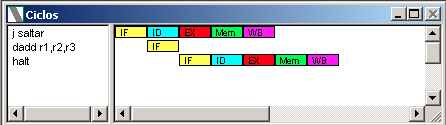
\includegraphics[scale=0.45]{atasco-branch-taken.png}
\end{block}
\end{frame}



\section{Posibles soluciones a problemas de dependencia de control}
\begin{frame}
\frametitle{General}
Existe una Penalización por salto, ya que se empieza a analizar la instrucción inmediata siguiente, mientras estamos decodificando el salto. Las instrución de salto puede ser: 
\begin{itemize}
\item Incondicional: La dirección de destino se debe determinar lo más pronto posible, dentro del cauce, para reducir la penalización.
\item Condicional: Introduce riesgo adicional por la dependencia entre la condición de salto y el resultado de una instrucción previa.
\end{itemize}
Deberiamos encontrar alguna manera de saber cual es la próxima instrucción lo antes posible.
\end{frame}


\subsection{Branch Target Buffer}
\begin{frame}
\frametitle{Branch-Target-Buffer}
Podemos ir guardando un historial de saltos para poder "predecir" si un salto se produce o no.

\begin{itemize}
\item No todos los saltos se pueden predecir. Solo los que tengan una dirección definida (jr depende del valor de un registro).
\item Cada vez que se ejecuta una instrucción de salto se guarda un registro si el salto se realizo o no (un registro para cada instrucción de salto). Ejemplo:
\begin{itemize}
\item Tengo un contador, inicialmente en 0. Sumo 1 por salto realizado, resto 1 si el salto no se realiza.
\item La próxima vez que pasé por esa instrucción puedo \emph{predecir} si el salto se realizará o no. 
\item Si el contador es positivo asumo se realizara el salto, la próxima instrucción será la que resulte de ejecutar el salto
\item Si el contador fuera negativo asumo no se realiza el salto, la próxima instrucción será la siguiente.
\end{itemize}
\item Que se hace la primera vez que se evalua un salto depende de la arquitectura.
\end{itemize}
\end{frame}

\begin{frame}
\frametitle{Branch-Target-Buffer en el Simulador}
\begin{itemize}
\item El simulador WinMIPS64 permite activar o desactivar la predicción de Saltos
\item La predicción de saltos usado en el simulador funciona de la siguiente manera:
\begin{itemize}
\item Si es la primera vez que se realiza el salto, se predice que el salto no va a ocurrir.
\item Si la instrucción se ejecuto por lo menos una vez, se asume que va a ocurrir lo último que ocurrió.
\item Si el resultado de la predicción cambio, se actualiza ese estado.
\end{itemize}
\item Si una predicción no ocurre, hay una penalidad de un ciclo perdido adicional.\end{itemize}
\end{frame}


\begin{frame}
\frametitle{Branch-Target-Buffer en el Simulador}
\begin{itemize}
\item Si un salto se predice que va a ocurrir y no ocurre. La penalidad son 2 atascos Branch Misprediction.
\item Si un salto se predice que no va a ocurrir y ocurre. La penalidad son 2 atascos Branch Taken.
\item Los 2 atascos corresponden a:
\begin{itemize}
\item 1 Ciclo para la actualización de la tabla BTB
\item 1 Ciclo para la carga de la nueva instrucción (como ocurria sin BTB)
\end{itemize}
\end{itemize}
\end{frame}

\begin{frame}
\frametitle{Branch-Target-Buffer en el Simulador}
\begin{itemize}
\item Si un salto se predice que va a ocurrir, podemos ver un simbolo después de la dirección de memoria en la ventana del programa
\end{itemize}
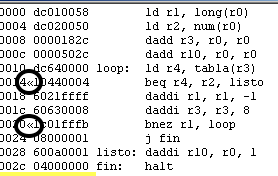
\includegraphics[scale=0.65]{btb.png}
\end{frame}


\subsection{Delay Slot}
\begin{frame}
\frametitle{Delay Slot}
Salto retardado o de relleno de ranura de retardo
\begin{itemize}
\item Es un método alternativo de atacar el problema de los atascos por dependencia de Control
\item El problema es la predicción de la siguiente instrucción luego de un salto.
\item Delay Slot ofrece como solución que la siguiente instrucción después de un salto \emph{SIEMPRE} se ejecute.
\item Esto elimina el problema de la predicción de instrucciones...
\item ... pero hay que tener en cuenta a la hora de programar.

\end{itemize}
\end{frame}

\begin{frame}[fragile]
\frametitle{Delay Slot}
¿Es lo mismo con o sin \emph{Delay Slot}?
\begin{block}{}
\begin{lstlisting}[basicstyle=\ttfamily,keywordstyle=\color{blue}]
       .data
A:   .word 2
       .code
       ld    r1, A(r0)
       daddi r2, r0, 3
       dadd  r3, r0, r0
salto: dadd  r3, r3, r1
       daddi r2, r2, -1
       bnez  r2, salto
       halt
\end{lstlisting}
\end{block}
\end{frame}


\begin{frame}[fragile]
\frametitle{Delay Slot - Solución 1 }
Podemos ``arreglar'' nuestro programa poniendo un \emph{NOP}, luego del salto.
\begin{block}{}
\begin{lstlisting}[basicstyle=\ttfamily,keywordstyle=\color{blue}]
       .data
A:   .word 2
       .code
       ld    r1, A(r0)
       daddi r2, r0, 3
       dadd  r3, r0, r0
salto: dadd  r3, r3, r1
       daddi r2, r2, -1
       bnez  r2, salto
       nop
       halt
\end{lstlisting}
\end{block}
\end{frame}


\begin{frame}[fragile]
\frametitle{Delay Slot - Solución 2 }
O podriamos reordenar las instrucciones...
\begin{block}{}
\begin{lstlisting}[basicstyle=\ttfamily,keywordstyle=\color{blue}]
       .data
A:   .word 2
       .code
       ld    r1, A(r0)
       daddi r2, r0, 3
       dadd  r3, r0, r0
salto: daddi  r2, r2, -1
       bnez  r2, salto
       dadd r3, r3, r1
       halt
\end{lstlisting}
\end{block}
\end{frame}


\begin{frame}
\frametitle{Delay Slot en el Simulador}
\begin{itemize}
\item El simulador WinMIPS64 permite activar o desactivar el Delay Slot
\item No se pueden tener activos Delay-Slot y Branch-Target-Buffer al mismo tiempo
\item Recordar que cualquier cambio en estas opciones involucra un reinicio en la simulación
\end{itemize}
\end{frame}


\end{document}
